% Template for Cogsci submission with R Markdown

% Stuff changed from original Markdown PLOS Template
\documentclass[10pt, letterpaper]{article}

\usepackage{cogsci}
\usepackage{pslatex}
\usepackage{float}

% amsmath package, useful for mathematical formulas
\usepackage{amsmath}

% amssymb package, useful for mathematical symbols
\usepackage{amssymb}

% hyperref package, useful for hyperlinks
\usepackage{hyperref}

% graphicx package, useful for including eps and pdf graphics
% include graphics with the command \includegraphics
\usepackage{graphicx}

% Sweave(-like)
\usepackage{fancyvrb}
\DefineVerbatimEnvironment{Sinput}{Verbatim}{fontshape=sl}
\DefineVerbatimEnvironment{Soutput}{Verbatim}{}
\DefineVerbatimEnvironment{Scode}{Verbatim}{fontshape=sl}
\newenvironment{Schunk}{}{}
\DefineVerbatimEnvironment{Code}{Verbatim}{}
\DefineVerbatimEnvironment{CodeInput}{Verbatim}{fontshape=sl}
\DefineVerbatimEnvironment{CodeOutput}{Verbatim}{}
\newenvironment{CodeChunk}{}{}

% cite package, to clean up citations in the main text. Do not remove.
\usepackage{cite}

\usepackage{color}

% Use doublespacing - comment out for single spacing
%\usepackage{setspace}
%\doublespacing


% % Text layout
% \topmargin 0.0cm
% \oddsidemargin 0.5cm
% \evensidemargin 0.5cm
% \textwidth 16cm
% \textheight 21cm

\title{A speed-accuracy tradeoff in children's processing of scalar
implicatures}


\author{{\large \bf Rose M. Schneider} \\ \texttt{rschneid@stanford.edu} \\ Department of Psychology \\ Stanford University \And {\large \bf Michael C. Frank} \\ \texttt{mcfrank@stanford.edu} \\ Department of Psychology \\ Stanford University}

\begin{document}

\maketitle

\begin{abstract}
Scalar implicatures---inferences from a weak description (``I ate some
of the cookies'') that a stronger alternative is not true (``I didn't
eat all'')---are a paradigm case of pragmatic inference. Children's
trouble with scalar implicatures is thus an important puzzle for
theories of the development of pragmatics, given their communicative
competence in other domains. Here, we explore children's reaction times
in a new paradigm for measuring scalar implicature processing. Alongside
falures on scalar implicature with ``some,'' we replicate previous
reports of failures on the quantifier ``none'' and find evidence of a
speed-accuracy tradeoff for both ``some'' and ``none.'' Motivated by
these findings, we use a Drift Diffusion Model to explore the
relationship between accuracy and reaction time in our task and find
evidence consistent with the hypothesis that preschoolers lack access to
the relevant alternatives for the scalar implicature computation. The
set of relevant alternatives may be broader than has been previously
assumed, however.

\textbf{Keywords:}
Pragmatics; development; scalar implicature; diffusion models.
\end{abstract}

\section{Introduction}\label{introduction}

Language comprehension in context is an inferetial process. Listeners
are not limited to interpreting the literal meaning of speakers'
utterances; they can also reason about what the speaker intended, based
on other utterances the speaker could have said. In the case of
\emph{pragmatic implicatures} (Grice, 1975), a speaker employs a weaker
literal description to imply that a stronger alternative is true. Adult
listeners tend to infer from the statement ``I enjoyed \emph{some} of my
winter break'' that some, but not all, of the break was pleasant. This
\emph{scalar implicature} (SI) relies heavily on a knowledge of the
relevant lexical alternatives in the quantifier scale \(<\)\emph{some},
\emph{all}\(>\). On standard theories, a listener must be able to
contrast ``some'' with the stronger descriptor ``all'' to compute the
implicature (Grice, 1975,Levinson (2000)).

SIs are challeinging for children until surprisingly late in development
(Noveck, 2001). For example, when judging a scene in which three of
three horses have jumped over a fence, five-year-olds are likely to
endorse the statement ``some of the horses jumped over the fence'' as
felicitous, despite the presence of a more informative alternative
(``all''; Papafragou \& Musolino, 2003). Children do seem to have some
knowledge of these scalar terms, however; for example, they reward
speakers based on the informativeness of their scalar descriptions
(Katsos \& Bishop, 2011). Given this early sensitivity, why do children
still struggle to compute scalar implicatures until late in development?

One possibile cause of children's failures is that they might not have
access to the relevant lexical alternatives (D. Barner \& Bachrach,
2010). This idea, which we will refer to as the \emph{Alternatives
Hypothesis}, predicts that if children cannot quickly and reliabily
bring to mind the relevant alternative quantifiers (e.g., ``all'' in a
situation where they hear ``some'') they will be unable to make the
implicature computation. The alternatives hypothesis makes a number of
predictions about children's abilities in reasoning about quantifiers,
some of which have been confirmed empirically. For example, consistent
with the idea of inaccessible alternatives, David Barner, Brooks, \&
Bale (2011) showed that four-year-olds could not even resolve the
quantifier expression ``only some'' (which should force alternatives to
be negated semantically, rather than pragmatically). But what are the
proper alternatives for SIs?

With respect to the proper set of alternatives for SI, the empirical
evidence has been changing rapidly. Although the conventional view on SI
is that the primary inferential alternative is ``all,'' a new body of
evidence suggests that more alternatives may be necessary---in
particular, ``none.'' For example, Degen \& Tanenhaus (2015) found that
set size changes the felicity of quantifier SIs for adults: ``some'' is
more felicitous when you couldn't say ``one'' or ``two.'' In a
computational reanalysis of these and other data, Franke (2014) showed
that a high weight on the alternative ``none'' was critical for fitting
these data. And in a recent study with children, Skordos \& Papafragou
(in press) found that exposing children to either ``all'' \emph{or}
``none'' facilitated their computation of subsequent SIs.

This relationship to ``none'' is unexpected on classic Gricean theories
(Grice, 1975, Horn (1972)), where the only alternatives should be those
logically entailed by the original message (i.e. ``all''). But it
\emph{is} in fact predicted by recent probabilistic models of
implicature. Under these models, all the relevant alternatives compete
with one another (M. C. Frank \& Goodman, 2012, Goodman \& Stuhlm{ü}ller
(2013), Franke (2014)). On the other hand, all of the evidence cited
above for the claim of ``none'' as an alternative is relatively
indirect, and such a substantial revision to standard theory requires
further evidence.

\begin{CodeChunk}
\begin{figure}[b]

{\centering 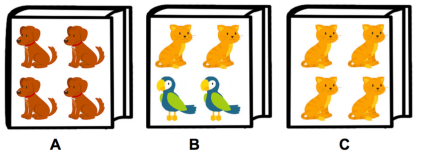
\includegraphics{figs/image-1} 

}

\caption[Example trial stimuli used in Horowitz and Frank (2015)]{Example trial stimuli used in Horowitz and Frank (2015).}\label{fig:image}
\end{figure}
\end{CodeChunk}

One other recent developmental study further supports the importance of
``none'' in SIs and provides the starting point for our current
experiment. Horowitz \& Frank (2015) designed a referent selection
paradigm that could be used across a broad age range (3--5 years) to
explore both scalar and ad-hoc (context dependent) implicatures. In this
task, children saw three book covers, each featuring four familiar
objects (Figure \ref{fig:image}). On target trials, the experimenter
described a book using a semantically ambiguous description (e.g., ``On
the cover of my book, some of the pictures are cats'' {[}scalar{]} or
``On the cover of my book are cats'' {[}ad hoc{]}). Children succeded on
ad-hoc trials but largely failed to make SIs, suggesting they had the
pragmatic competence necessary to compute the implicature.

Interestingly, in Horowitz \& Frank (2015), the same children who failed
on SI also failed on unambiguous ``none'' control trials---and in
several samples, performance was highly correlated between ``none'' and
``some'' trials. This result would be predicted if ``none'' was in fact
an inferential alternative. If some children were not computing its
semantics appropriately in an online fashion, they would be the children
to fail in the SI computation as well.

One further prediction of the alternatives hypothesis relates to
processing time. Perhaps children who have a fully-established
quantifier scale---and hence can make correct SIs---take additional time
in using this information, due to competition between alternatives.
Congruent with this prediction, our intuition in the Horowitz \& Frank
(2015) study described above and in pilot studies using this same
paradigm was that when children made correct SIs they appeared to be
taking longer than when they failed. But although reaction time measures
have been commonplace in studies of adults' SI processing, they have
been almost entirely absent in the developmental literature (with the
exception of Huang \& Snedeker, 2009, whose data showed little evidence
of SI computation).

Thus, in our current study, we explore children's behavioral response
latencies in an iPad adaptation of the Horowitz \& Frank (2015) scalar
implicature task. In our analyses, we explore overall accuracy and
patterns of performance, as in (Horowitz \& Frank, 2015), and find that
children not only struggle in making a scalar implicature, but replicate
the finding that they also grapple with ``none'' until fairly late in
development. Congruent with our predictions, in examining reaction time
patterns across all quantifier types, we find evidence of a
speed-accuracy tradeoff for both quantifiers. Finally, we use a Drift
Diffusion Model to explore the source of this increased reaction time.
Overall, our findings are consistent with a version of the Alternatives
Hypothesis under which ``none'' is an important inferential alternative
in SI and its availability causes slower processing times but correct
SIs. We consider this and other alternative explanations in the
Discussion.

\section{Method}\label{method}

In this study, we adapted the scalar implicature paradigm developed by
Horowitz \& Frank (2015) for the iPad. In addition to capturing detailed
reaction time data, this version included more trials, and standardized
prosody across all trials, as well as a completely randomized
design.\footnote{The full experiment can be viewed online at \texttt{https://rosemschneider.github.io/tablet\_exp/si\_tablet.html} and all of our data, processing, experimental stimuli, and analysis code can be viewed in the version control repository for this paper at: \texttt{https://github.com/rosemschneider/SI\_tablet}.}

\subsection{Participants}\label{participants}

\begin{table}[t]
\centering
\begin{tabular}{c c c c c } 
 \hline
 Age group & N & Mean & Median & SD \\
 \hline
 3--3.5 years & 24 & 3.27 & 3.27 & 0.14\\
 3.5--4 years & 35 & 3.78 & 3.73 & 0.15 \\ 
 4--4.5 years & 25 & 4.28 & 4.28 & 0.15\\
 4.5--5 years & 30 & 4.76 & 4.76 & 0.15 \\
 5--6.5 years & 24 & 5.55 & 5.56 & 0.36 \\
 \hline
\end{tabular}
\caption{Age information for all participants.}
\label{tab:age}
\end{table}

Table \ref{tab:age} shows the breakdown of age information for all
participants. Included in analyses are 138 children out of a planned
sample of 120 participants, recruited from both a local daycare and a
local children's museum. We ran 20 additional children, who were
excluded from analysis based on planned exclusion criteria of low
English language exposure (\(\leq 75\%\)) or \(<50\%\) of trials
completed. Included in our sample were 79 females and 59
males.\footnote{Based on Horowitz \& Frank (2015), we initially planned
  to collect data from children 3--5 years. After collecting data from
  57 participants, however, we observed significantly lower performance
  on implicature trials across all age groups, indicating that the iPad
  adaptation of the scalar implicature task was slightly more
  challenging for all children, and included an older age group of 24
  5--6.5-year-olds.}

\subsection{Stimuli and design}\label{stimuli-and-design}

The general format of the task was identical to Horowitz \& Frank
(2015), with the exception of added items for additional trials. The
study was programmed in HTML, CSS, and JavaScript, and displayed to
children on a full-sized iPad. Each trial displayed three book covers,
each containing a set of four familiar objects (Figure \ref{fig:image}).
Each session involved 30 trials, with 10 trials per quantifier-type
(``all'', ``some'', and ``none''). Each audio clip used the same three
initial sentence frames (e.g., ``On the cover of my book, \emph{some} of
the pictures\ldots{}'') so that prodosdy was emphasized equally across
all trials. The average length of each audio clip (including target item
phrase, e.g., ``\ldots{}are cats'') was approximately 6s. In our
randomization, quantifier triad order, items (within category), target
item, and quantifier were randomized for all participants. In all, there
were 270 different target items and audio clips.

\subsection{Procedure}\label{procedure}

Sessions took place individually in a small testing room away from the
museum floor or the classrooom of the daycare. To familiarize children
with the iPad, each session began with a ``dot game,'' which required
them to press dots on the screen as fast as possible. After the dot
game, the experimenter introduced them to ``Hannah,'' a cartoon
character who wanted to play a guessing game with her books. The
experimenter explained that Hannah would show the child three books, and
would give one hint about which book she had in mind, so they had to
listen carefully. Children then saw a practice trial with an unambiguous
noun referent.

Each trial allowed 2.5s for children to visually inspect the three book
covers, before the experiment played the trial prompt (e.g., ``On the
cover of my book, \emph{none} of the pictures are cats.''). Reaction
times were measured from the onset of the target word. Children could
only make one selection. If a child was not paying attention, or if she
did not hear Hannah's prompt, the experimenter repeated it, matching the
original prosody. Once children correctly made their selection, a green
box appeared around the chosen book. The experiment was self-paced, and
children initiated each trial by pressing a button that appeared after
they had made their selection in the previous trial.

\begin{CodeChunk}
\begin{figure}[t]
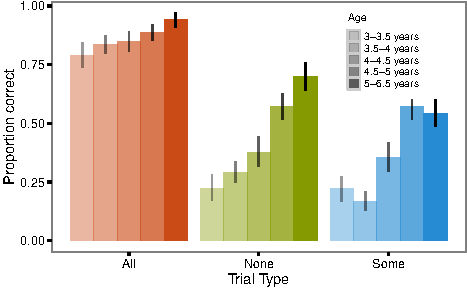
\includegraphics{figs/overall_acc-1} \caption[Children's overall accuracy for each quantifier type]{Children's overall accuracy for each quantifier type. Bars show mean performance for each age group. Error bars are 95 percent confidence intervals computed by non-parametric bootstrap.}\label{fig:overall_acc}
\end{figure}
\end{CodeChunk}

\section{Results}\label{results}

To exclude trials where the child had missed the prompt or was not
paying attention, we excluded reaction times (RTs) longer than 15s.
After this initial cut, we excluded RTs outside three standard
deviations of the log of mean reaction time. This cleaning process
resulted in a data loss of 85 trials (2.14\%).

\subsection{Accuracy}\label{accuracy}

Figure \ref{fig:overall_acc} shows children's for each trial type, split
by age group. For each age group, we saw significantly lower accuracy
for the quantifiers ``some'' and ``none'' in comparison to ``all'' (all
\(p\)s \(< .01\) in two-sample t-tests for each age group). These
results generally replicate our previous findings using this paradigm
(Horowitz \& Frank, 2015), but one difference from the previous results
was in implicature trials. Children aged 3--5 years performed
significantly lower on ``some'' (implicature) trials in this task in
comparison with data from Horowitz, Schneider, \& Frank (in prep.)
(\(p < .01\) for all tests). Thus, while the iPad adaptation was
generally successful, implicatures were more difficult, perhaps because
of the non-social nature of the iPad interaction or the recorded audio
stimuli.

\begin{CodeChunk}
\begin{figure}[t]
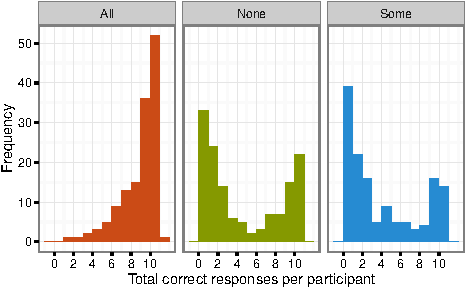
\includegraphics{figs/diptest-1} \caption[Frequency histogram of correct responses for each trial type, across all participants]{Frequency histogram of correct responses for each trial type, across all participants.}\label{fig:diptest}
\end{figure}
\end{CodeChunk}

\begin{CodeChunk}
\begin{figure*}[t]

{\centering 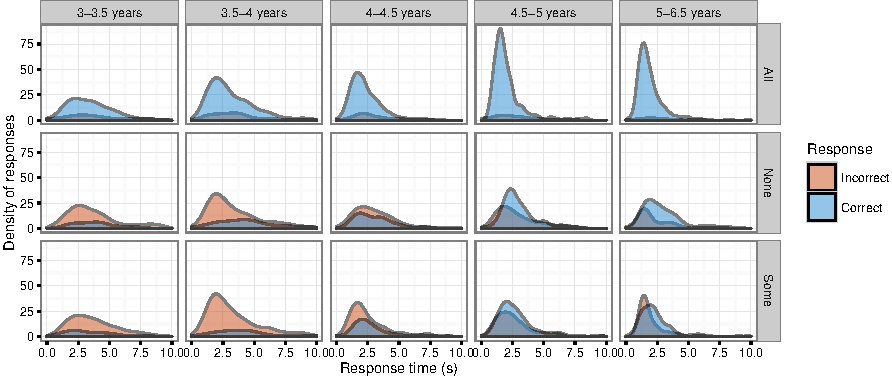
\includegraphics{figs/dense-1} 

}

\caption[Density plots of reaction times for correct and incorrect responses on each trial type, split by age]{Density plots of reaction times for correct and incorrect responses on each trial type, split by age.}\label{fig:dense}
\end{figure*}
\end{CodeChunk}

We next fit a logistic mixed effects model predicting correct response
as an interaction of age and trial type, with random effects of trial
type and
participant.\footnote{All mixed effects models were fit in \texttt{R} using the \texttt{lme4} package. The model specification was: \texttt{correct ~ age * trial type + (trial type | subject id)}.}
Performance was significantly lower on ``some'' (\(\beta = -6.98\),
\(p < .0001\)) and ``none'' trials (\(\beta = -9.55\), \(p < .0001\)).
There was also a signficant interaction between age and trial type on
``none'' trials (\(\beta\) = 1.53, \(p\) \textless{} .0001), indicating
that children's performance with this difficult quantifier increased
with age.

Figure \ref{fig:diptest} shows distributions of correct responses for
all trial types. Performance on ``some'' and ``none'' trials was bimodal
(Hartigan's \(D\) = 0.08, \(p\) \textless{} .0001) and ``none'' trials
(\(D\) = 0.11, \(p\) \textless{} .0001). While children's average
accuracy was low for these quantifiers, there were some children who
were correct on the majority of these trials (``Some'': N = 28;
``None'': N = 36) and the others were typically incorrect on the
majority of trials. Children did not appear to be responding randomly.
As in previous work, we found a strong correlation between children's
accuracy on ``some'' and ``none'' trials (\(r\) = 0.49, \(p\)
\textless{} .0001).

\subsection{Reaction time}\label{reaction-time}

We fit a linear mixed effects model predicting log RT on correct trials
as a function of log trial number, the interaction of age and trial
type, and random effects of trial type by subject.\footnote{Model
  specification:
  \texttt{log(reaction time) ~ log(trial number) + age * trial type + (trial type | subject id)}.
  Age was centered for ease of interpretation of coefficients, and we
  calculated \emph{p} values via the \(t=z\) approximation.} Reaction
times were longer on ``none'' (\(\beta = 0.22\), \(p < .0001\)) and
``some'' trials (\(\beta = 0.1\), \(p < .0001\)), and reaction times
decreased with age (\(\beta = -0.1\), \(p < .0001\)). There were no
significant interactions between age and trial type. The model also
showed a main effect of trial number, with reaction times decreasing
over the course of the study (\(\beta\) = -0.27, \(p\) \textless{}
.00001).

Examination of the pattern in Figure \ref{fig:dense} suggests that
accuracy and reaction time may be interacting, however. In particular,
while correct responses on ``all'' trials appear to be faster than the
(few) incorrect responses, the opposite is true for ``none'' and
``some'' trials: Errors have faster RTs, potentially indicating a
speed-accuracy tradeoff. To test for this effect, we fit another mixed
effects model, this time including accuracy and its interactions with
age and trial type as predictors. This model revealed that correct
trials overall had faster RTs (\(\beta = -0.16\), \(p = .0002\)), but
that this accuracy term interacted negatively with trial type such that
both ``none'' and ``some'' trials had slower RTs for correct trials
(\(\beta = 0.34\), \(p < .0001\); \(\beta = 0.27\), \(p < .0001\)).
There were no three-way interactions of trial-type and age. This model
thus provides evidence of a speed-accuracy tradeoff for ``some'' and
``none'' trials.

We fit a linear mixed effects model predicting log RT on correct trials
as a function of log trial number, the interaction of age and trial
type, and random effects of trial type by subject.\footnote{Model
  specification:
  \texttt{log(reaction time) ~ log(trial number) + age * trial type + (trial type | subject id)}.
  Age was centered for ease of interpretation of coefficients, and we
  calculated \emph{p} values via the \(t=z\) approximation.} Reaction
times were longer on ``none'' (\(\beta = 0.38\), \(p < .0001\)) and
``some'' trials (\(\beta = 0.22\), \(p < .0001\)), and reaction times
decreased with age (\(\beta = -0.29\), \(p < .0001\)). There were no
significant interactions between age and trial type. The model also
showed a main effect of trial number, with reaction times decreasing
over the course of the study (\(\beta\) = -0.1, \(p\) \textless{}
.00001).

Examination of the pattern in Figure \ref{fig:dense} suggests that
accuracy and reaction time may be interacting, however. In particular,
while correct responses on ``all'' trials appear to be faster than the
(few) incorrect responses, the opposite is true for ``none'' and
``some'' trials: Errors have faster RTs, potentially indicating a
speed-accuracy tradeoff. To test for this effect, we fit another mixed
effects model, this time including accuracy and its interactions with
age and trial type as predictors. This model revealed that correcvt
trials overall had faster RTs (\(\beta = -0.16\), \(p = .0002\)), but
that this accuracy term interacted negatively with trial type such that
both ``none'' and ``some'' trials had slower RTs for correct trials
(\(\beta = 0.34\), \(p < .0001\); \(\beta = 0.27\), \(p < .0001\)).
There were no three-way interactions of trial-type and age. This model
thus provides evidence of a speed-accuracy tradeoff for ``some'' and
``none'' trials.

\subsection{Drift diffusion models}\label{drift-diffusion-models}

Our preliminary analysis of children's reaction times in this task
indicated greater response latencies associated with success on ``some''
and ``none'' trials. Motivated by these patterns, we explored the
interaction between reaction time and accuracy in more depth with a DDM.
A DDM can be used in behavioral tasks to provide a more detailed view of
the relationship between accuracy and reaction time (Milosavljevic,
Malmaud, Huth, Koch, \& Rangel, 2010; Ratcliff \& Rouder, 1998).

In DDM, a behavioral response (a correct or incorrect choice) is the
result of noisy data accumulation through a diffusion process (Ratcliff
\& Rouder, 1998). Responses have \emph{separation boundaries} that are
dependent on the amount of information needed to initate a response, and
\emph{drift rate} formalizes the rate of data accumulation (Ratcliff \&
Rouder, 1998). \emph{Nondecision} is the amount of time between stimuli
offset, and initiating the diffusion process. Finally, different
responses may have a \emph{bias}, or different starting point in the
diffusion process, dependent on the stimuli (Ratcliff \& Rouder, 1998).

Although a DDM is traditionally fit to data from two-alternative
forced-choice tasks, here we estimate the drift process between a
correct and incorrect choice, with two options in each trial being
``incorrect,'' and only one being consistent with the target noun and
quantifier. In fitting a DDM to our data in this way, we estimated
parameters for each subject across all three trial types (``all'',
``some'', and ``none'') using the RWiener package. We then aggregated
across subjects to obtain means and confidence intervals for each age
group. Figure \ref{fig:devo_param_plot} shows the parameter estimates
for each age group, split by trial type.

\begin{CodeChunk}
\begin{figure*}[t]

{\centering 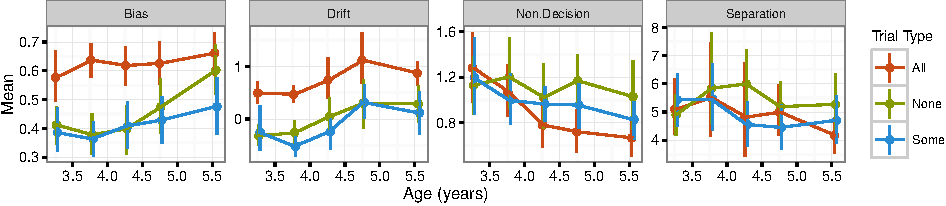
\includegraphics{figs/devo_param_plot-1} 

}

\caption[Parameter estimates for drift diffusion model, split by age and trial type]{Parameter estimates for drift diffusion model, split by age and trial type. Error bars are 95 percent confidence intervals computed by nonparametric bootstrap.}\label{fig:devo_param_plot}
\end{figure*}
\end{CodeChunk}

For each estimate, we ran a mixed effects model, predicting parameter
value as an interaction of age and trial
type.\footnote{The specifications for all parameter models are as follows: \texttt{Parameter Value ~ age * trial type + (1 | subject ID)}}
In our separation boundary estimates, there was no significant effect of
trial type on boundary estimates, indicating that roughly the same
amount of information needs to be accumulated to make a decision in each
trial type. In our nondecision parameter estimates, we found a
significant main effect of age (\(\beta\) = -0.28, \(p\) \textless{}
.00001), as well as a interaction between age and ``none'' trials
(\(\beta\) = 0.24, \(p\) = .01).

As expected in drift rate, there was negative main effect of trial type
(``None'': \(\beta\) = -1.3, \(p\) = .0185; ``Some'': \(\beta\) = -1.18,
\(p\) = .03) Interestingly, in our bias estimates the model revealed a
significant negative effect of ``none'' trials (\(\beta\) = -0.5, \(p\)
= .0005), and ``some'' trials showed borderline significance (\(\beta\)
= -0.28, \(p\) = .0503), as well as a significant interaction between
age and ``none'' trials (\(\beta\) = 0.07, \(p\) = .023).

Taken together, the parameter estimates from our DDM indicate that as
children develop (and become more familiar with the quantifier scale),
they are more likely to respond correctly in our scalar implicature
task, while younger children fail, due to a low rate of data
accumulation and a high separation boundary. Interestingly, children's
bias increases across development for ``none,'' but not for ``some,''
possibly because ``none'' strength as a competitor for ``some''
increases with increased access to alternatives.

It is possible that meaningful differences in the diffusion process
might be revealed by accounting for accuracy. In an exploratory
analysis, we use accuracy on scalar implicature trials to independently
estimate parameters for participants. We split children by accuracy on
scalar implicature trials, and then estimated parameters by accuracy
group. High accuracy was defined as an average of 75\% performance on
scalar implicature trials. Figure \ref{fig:param_plot} shows the
paramter estimates for each accuracy group, split by trial type.

\begin{CodeChunk}
\begin{figure*}[t]

{\centering 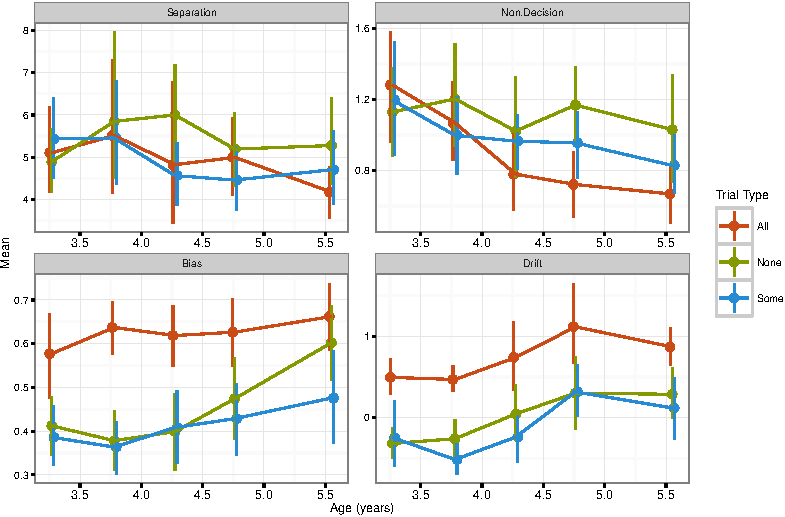
\includegraphics{figs/param_plot-1} 

}

\caption[Parameter estimates for drift diffusion model, split by accuracy and trial type]{Parameter estimates for drift diffusion model, split by accuracy and trial type. Error bars are 95 percent confidence intervals computed by nonparametric bootstrap.}\label{fig:param_plot}
\end{figure*}
\end{CodeChunk}

As in our developmental DDM, we did not find any significant effects of
separation or nondecision. While drift rates show a significant effect
of accuracy, because we estimated parameters for high and low accuracy
children separately, these are defined by the analysis.

In our bias estimates, however, we found a significant interaction
between accuracy group and trial type on ``some'' trials (\(\beta\) =
-0.18, \(p\) = .0013). This interaction suggests that bias (the starting
point in the diffusion process) might be an important factor in
successfully making a scalar implicature. When we included an age
coefficient in this model, this interaction was no longer significant;
instead, we found a significant interaction between age, trial type
``some'', and accuracy (\(/beta\) = -0.18, \(p\) = .024).

While it seems that when accounting for age children's bias on ``some''
trials is not affected by scalar implicature accuracy, older children in
the low accuracy group are significantly more likely to have a lower
bias for ``some.'' This observed interaction, together with the findings
of our previous accuracy models, does provide evidence for the
availability of ``none'' providing a salient alternative that results in
a speed-accuracy tradeoff in making a scalar implicature.

\section{General Discussion}\label{general-discussion}

Our primary question in this study centered on whether success in making
scalar implicatures requires increased response latencies to make use of
relevant scalar alternatives. We adapted a previously validated scalar
implicature task (Horowitz \& Frank, 2015; Horowitz et al., in prep.)
for the iPad to explore the relationship between reaction time and
accuracy.

In our analyses, we replicated previous patterns of performance in
Horowitz \& Frank (2015) and Horowitz et al. (in prep.). We found that
children were overall less accurate when evaluting the quantifiers
``some'' and ``none'' in comparison to ``all,'' but that their
performance increased over development. We again found evidence of
bimodal and correlated performance on these two quantifier types,
suggesting a common source of difficulty. Additionally, we discovered in
a statistical model that although children were more likely make an
incorrect response on ``some'' and ``none'' trial, their performance on
these trials signficantly increased with age.

In our extension of this paradigm, we collected reaction time data for
these quantifier types to investigate the relationship between reaction
time and accuracy. In our reaction time analyses, we found evidence of a
speed-accuracy tradeoff, as well as an interaction between reaction time
and age, with older children taking a slightly longer time to respond to
these trials, but ultimately being more accurate. These findings
motivated our decision to fit our data to a Drift Diffusion Model.

As an exploratory analysis, we fit a DDM to our data to prediction the
relationship between reaction time and accuracy for children who succeed
in making scalar implicatures versus children who fail. While the
results are preliminary, we found some evidence that bias might be a
critical factor in success in making a scalar implicature.
Interestingly, this effect seems to be driven by age, such that older
children who fail on these trials have significantly lower bias in
comparison to ``all'' trials. It is very likely that the high
variability and wide distribution of reaction times observed in this
study contributed to the unclear findings observed in our DDM. Given
that we did see indications that bias is a significant part of
successfully making a scalar implicature, however, future work should
explore this relationship.

Our work contributes to the existing literature in utilizing a novel
method to collect accurate and detailed reaction time data on a scalar
implicature task. Response latencies are an important indicator of the
pragmatic challenges that children face in processing implicatures.
Additionally, our findings replicate previous work, providing evidence
for the appropriateness of this paradigm in targeting scalar
implicatures. Further, our larger sample size, increased number of
trials, and randomized design strengthen our analytical power, and allow
for more detailed inferences from the data. Our work supports not only
the hypthesis that children must be familiar with the quantifier scale
in order to make an implicature, but also provides preliminary evidence
that doing correctly doing so may require additional processing time.

Taken together, our work suggests that there is a meaningful
relationship between children's accuracy and reaction times in making
scalar implicatures throughout development. From our results, the
relationship between children's quantifier knowledge, processing speed,
and scalar implicature computation is unclear, and future work should
test these links more explicitly. Our work suggests, however, that
comparing a speaker's statement to possible alternatives in order to
make an implicature is an active process for children, and does seem to
result in a speed-accuracy tradeoff.

\section{Acknowledgements}\label{acknowledgements}

Thanks to Bing Nursery School and the San Jose Children's Discovery
Museum. Thanks also to Veronica Cristiano, Rachel Walker, and Tamara
Mekler for their help with data collection, and to Kara Weisman and Ann
Nordmeyer for their assistance creating stimuli.

\section{References}\label{references}

\setlength{\parindent}{-0.1in} \setlength{\leftskip}{0.125in} \noindent

Barner, D., \& Bachrach, A. (2010). Inference and exact numerical
representation in early language development. \emph{Cognitive
Psychology}, \emph{60}(1), 40--62.

Barner, D., Brooks, N., \& Bale, A. (2011). Accessing the unsaid: The
role of scalar alternatives in children’s pragmatic inference.
\emph{Cognition}, \emph{118}(1), 84--93.

Degen, J., \& Tanenhaus, M. K. (2015). Processing scalar implicature: A
constraint-based approach. \emph{Cognitive Science}, \emph{39}(4),
667--710.

Frank, M. C., \& Goodman, N. D. (2012). Predicting pragmatic reasoning
in language games. \emph{Science}, \emph{336}(6084), 998--998.

Franke, M. (2014). Typical use of quantifiers: A probabilistic speaker
model. In \emph{Proceedings of the 36th annual conference of the
cognitive science society} (pp. 487--492).

Goodman, N. D., \& Stuhlm{ü}ller, A. (2013). Knowledge and implicature:
Modeling language understanding as social cognition. \emph{Topics in
Cognitive Science}, \emph{5}(1), 173--184.

Grice, H. P. (1975). Logic and conversation. In P. Cole \& J. Morgan
(Eds.), \emph{Syntax and semantics} (Vol. 3). New York: Academic Press.

Horn, L. R. (1972). \emph{On the semantic properties of logical
operators.} (PhD thesis). University of California, Los Angeles.

Horowitz, A., \& Frank, M. C. (2015). Sources of developmental change in
pragmatic inferences about scalar terms. In \emph{Proceedings of the
37th annual conference of the cognitive science society.}

Horowitz, A., Schneider, R. M., \& Frank, M. C. (in prep.). The trouble
with quantifiers: Children's difficulties with ``some'' and ``none''.

Huang, Y. T., \& Snedeker, J. (2009). Online interpretation of scalar
quantifiers: Insight into the semantics-pragmatics interface.
\emph{Cognitive Psychology}, \emph{58}(3), 376--415.

Katsos, N., \& Bishop, D. (2011). Pragmatic tolerance: Implications for
the acquisition of informativeness and implicature. \emph{Cognition},
\emph{120}(1), 67--81.

Levinson, S. C. (2000). \emph{Presumptive meanings: The theory of
generalized conversational implicature}. MIT Press.

Milosavljevic, M., Malmaud, J., Huth, A., Koch, A., \& Rangel, A.
(2010). Drift diffusion model can account for accuracy and reaction time
of value-based choices under high and low time pressure. \emph{Judgment
and Decision Making}, \emph{5}(6), 437--449.

Noveck, I. (2001). When children are more logical than adults:
Experimental investigations of scalar implicature. \emph{Cognition},
\emph{78}(2), 165--188.

Papafragou, A., \& Musolino, J. (2003). Scalar implicatures: Experiments
at the semantics-pragmatics interface. \emph{Cognition}, \emph{86}(3),
253--282.

Ratcliff, R., \& Rouder, J. (1998). Modeling response times for
two-choice decisions. \emph{Psychologial Science}, \emph{9}(5),
347--356.

Skordos, D., \& Papafragou, A. (in press). Children's derivation of
scalar implicatures: Alternatives and relevance. \emph{Cognition}.

\end{document}
